% ----------------------------------------------    
% ----------------------------------------------
\smallsection{Dependence of label noise in adversarial training}
\label{sect:dependence-label-noise}
    % We now show the implicit label noise in adversarial training depends on the perturbation radius and the data quality given mild assumptions on the probabilistic classifier.
    % and show how these factors affect double descent in adversarial training.
    % \begin{corollary}[Dependence of implicit label noise]
    % % Assume the true label distribution $P(Y^*|x)$ is locally convex around $x$ and can be asymptotically described as
    % % \chengyu{Twice differentiable is also enough. Use Taylor approximate in first order to express gradient with perturbed distance. But here need to show it is negative correlation, meaning norm after hessian multiplication is negative correlated}
    % Assume $f(x)_y$ is $L$-locally Lipschitz around $x$ with Hessian bounded below. Let $m = \inf_{z \in \mathcal{B}_\varepsilon(x)} \sigma_{\min} (\nabla^2 f(z)_y) > 0$, we have
    % \begin{equation}
    % \label{theo:label-noise-dependence}
    %     % \|p_Y - p_{Y'}\|_{\text{TV}} 
    %     P(\tilde{Y’}\ne Y' | x')
    %     \ge
    %     \frac{\varepsilon}{2} (1 - q(x)) \frac{m}{L}  - \frac{\varepsilon^2}{4} M,
    % \end{equation}
    % where $q(x)$ is the data quality.
    % % \begin{equation}
    % % \label{eq:label-noise-assumption}
    % %     %  \|\nabla_x~ p(y^*=j|x)\| \propto 
    % %     % \begin{cases}
    % %     % 1 -  p(y^*=j|x),& \quad  p(y^*=j|x) \to 1\\
    % %     %      p(y^*=j|x),& \quad  p(y^*=j|x) \to 0,
    % %     % \end{cases}   
    % %      \|\nabla_x~ P(Y^*=j|x)\| \propto 1 -  P(Y^*=j|x),
    % % \end{equation}
    % % as $P(Y^*=j|x) \to 1$.
    % % % $\max_j p(y^*=j|x) \approx 1$, % Given in assumption
    % % % where $j^* = \argmax~p(y=j|x)$, given by above lemma 2.2
    % % We have
    % % $$
    % % \underline{\min}~P(\tilde{Y}_\delta \ne Y^*_\delta | x_\delta) \propto \varepsilon (1 - q(x)),
    % % $$
    % % where $\underline{\min}$ means the lower bound of the minimum label noise, and $q(x)$ is the data quality (\ref{definition:data-quality}).
    % \end{corollary}
    % \begin{proof}
    % % See Appendix~\ref{sect:label-noise-more-proof}, where we also show that Assumption (\ref{eq:label-noise-assumption}) holds true for a Gaussian mixture model.
    % Let $f(x) = f(x)_y$. Assume $f$ is locally Lipschitz around $x$. Let $x^* = \argmin_{z \in X, f(z) = 1} \|x - z\|$ (local maximum closest to $x$). Because $x^*$ is the local maximum and $f$ is continuously differentiable, $\nabla f(x^*) = 0$, thus
    % $$
    % \nabla f(x) 
    % & = \nabla f(x^*) + \nabla^2 f(z) (x - x^*) = \nabla^2 f(z) (x - x^*).
    % $$
    % Therefore we have
    % $$
    % \begin{aligned}
    % \|\nabla f(x)\| 
    % & =  \|\nabla^2 f(z) (x - x^*) \| \\
    % & \ge \sigma_{min} (\nabla^2 f(z)) \|x - x^*\| \\
    % & \ge \sigma_{min} (\nabla^2 f(z)) \frac{|f(x^*) - f(x)|}{L(f)} \\
    % & = \frac{\sigma_{min} (\nabla^2 f(z))}{L(f)} |1 - f(x)| \\
    % & = \frac{\sigma_{min} (\nabla^2 f(z))}{L(f)} |1 - q(x)| \\
    % \end{aligned}
    % $$
    % \end{proof}
    % The above theorem shows that, % when the data quality of the clean example is relatively high,
    % the probability of the true label of the clean example is relatively high, 
    Theorem~\ref{theo:main} shows that
    the label noise in adversarial training is proportional to (1) the perturbation radius (2) the data quality. 
    % Larger perturbation radius and low data quality induces higher implicit label noise, which echos the empirical observations made in Appendix~\ref{sect:double-descent-adversarial}.
    % Since implicit label noise modulates the double descent, and by Theorem~\ref{theo:label-noise-perturbation} it depends on the perturbation radius and data quality, the double descent in adversarial training should strongly correlate with the perturbation radius and data quality. 
    % Indeed, it has been observed respectively that small perturbation radius will not induce robust overfitting~\citep{Dong2021ExploringMI}, and high-quality data will not induce robust overfitting~\citep{Dong2021DataPF}.
    % , which will subsequently affect the double descent curves.
    Considering label noise can be an important source of variance in the generalization of deep neural networks~\citep{Nakkiran2020DeepDD, Yang2020RethinkingBT}, such dependence of label noise explains the intriguing observations in the literature that robust overfitting (or epoch-wise double descent) in adversarial training will vanish with small perturbation radii~\citep{Dong2021ExploringMI} or high-quality data~\citep{Dong2021DataPF}. 
    We conduct more controlled experiments to verify this correlation empirically, as shown in Figure~\ref{fig:dependence-perturbation-quality}, 
    % More controlled experiments are conduct in Appendix~\ref{sect:double-descent-adversarial} to verify this correlation empirically.
    
    \begin{figure*}[!ht]
      \centering
      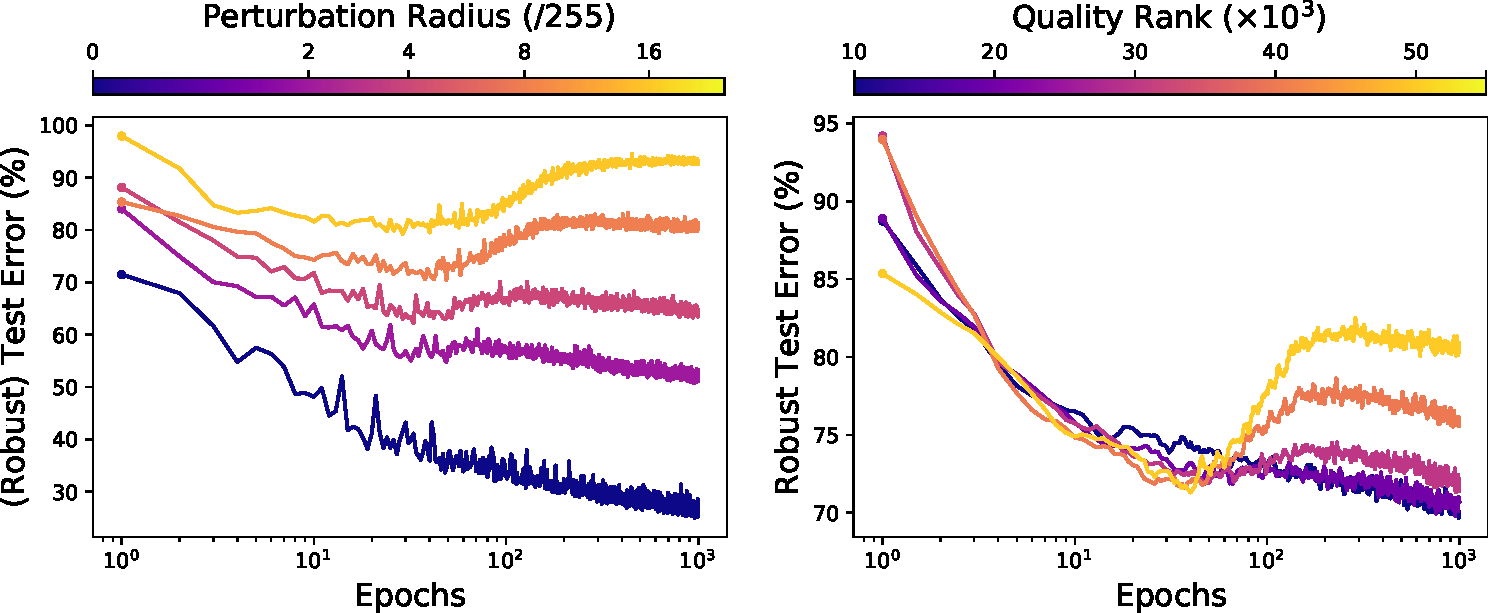
\includegraphics[width=0.8\textwidth]{figures/dependence-perturbation-quality.pdf}
      \caption{(Left) Dependence of robust overfitting on the perturbation radius. A training subset of size 5k is randomly sampled to speed up the training.
      % As the perturbation radius (used for both training and testing) employed in adversarial training increases, both the epoch-wise and model-wise double descent become more prominent.
      $\varepsilon = 0/255$ indicates the standard training where no double descent occurs. 
      (Right) Dependence of robust overfitting on the data quality with a fixed perturbation radius ($\varepsilon = 8/255$). To construct a training subset with high data quality, we first calculate the predictive probability based on an ensemble of multiple models. We then rank all training examples based on the predictive probability and select the top-k ones.
      The curves are smoothed by a window of $5$ epochs to reduce overlapping.
      Here we conduct PGD training on CIFAR-10 with WRN-28-5. 
      More experiment details can be found in the Appendix. % ~\ref{sect:double-descent-adversarial}.
      % As the quality of training data in adversarial training degrades, both the epoch-wise and model-wise double descent become more prominent. In the epoch-wise double descent figure, We smooth each curve by a window of 5 epochs to reduce the overlapping area. For the model-wise double descent the test error at the last checkpoint (solid line) and the test error at the best checkpoint (dashed line) are both shown. 
    %   \chengyu{change data quality to $1 - f_\theta(y|x)$}
      }
      \vspace{-1em}
    \label{fig:dependence-perturbation-quality}
    \end{figure*}